%\documentclass[10pt,dvipdfmx]{article}
%\usepackage{pgf,tikz}
%\usepackage{mathrsfs}
%\pagestyle{empty}
%\begin{document}
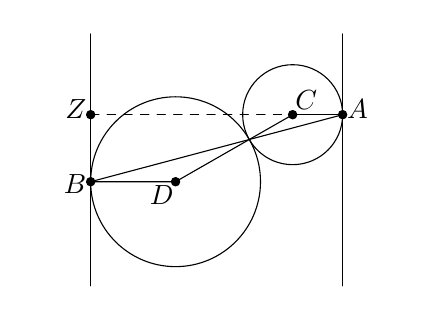
\begin{tikzpicture}[line cap=round,line join=round,x=0.4cm,y=0.4cm]
\clip(-6,-4.2) rectangle (6,4.2);
\draw (4,4)-- (4,-4);
\draw (-4,4)-- (-4,-4);
\draw[fill=black](-1.303812,-0.6909094) circle  (1.5pt);
\draw[fill=black](-1.745614,-1.1250269) node  {$D$};
\draw(-1.303812,-0.6909094) circle (2.696188);
\draw[fill=black](2.413071,1.437441) circle  (1.5pt);
\draw[fill=black](2.842632,1.893326) node  {$C$};
\draw(2.413071,1.437441) circle (1.586929);
\draw[fill=black](-4.000001,-0.6909105) circle  (1.5pt);
\draw[fill=black](-4.492705,-0.7760141) node  {$B$};
\draw (-4.000001,-0.6909105)-- (-1.303812,-0.6909094);
\draw[fill=black](4.000001,1.437443) circle  (1.5pt);
\draw[fill=black](4.470541,1.606536) node  {$A$};
\draw (2.413071,1.437441)-- (4.000001,1.437443);
\draw (-1.303812,-0.6909094)-- (2.413071,1.437441);
\draw (-4.000001,-0.6909105)-- (4.000001,1.437443);
\draw[fill=black](-4.000001,1.437438) circle  (1.5pt);
\draw[fill=black](-4.470541,1.606531) node  {$Z$};
\draw [dashed](-4.000001,1.437438)-- (2.413071,1.437441);
\end{tikzpicture}
%\end{document}
